\documentclass[aspectratio=169]{beamer}
\usetheme{arguelles}
\usepackage{tikz}
\usepackage{pgfplots}
\usepackage{amsmath}
\usepackage{graphicx}
\usepackage{booktabs}

\title{Dialysis: DTMF Signal Analysis Studio}
\subtitle{Algorithms, Signal Processing, and Real-Time Decoding}
\author{Antigravity}
\date{\today}

\begin{document}

\frame[plain]{\titlepage}

\begin{frame}{What is DTMF?}
    \textbf{Dual-Tone Multi-Frequency (DTMF)} is the global standard for telecommunication signaling over analog telephone lines in the voice-frequency band.
    
    \vspace{0.5cm}
    \begin{columns}
        \begin{column}{0.5\textwidth}
            \textbf{How it works:}
            \begin{itemize}
                \item Each key press generates \textbf{two} simultaneous pure sine waves.
                \item One from a \textit{low-frequency} group (rows).
                \item One from a \textit{high-frequency} group (columns).
            \end{itemize}
        \end{column}
        \begin{column}{0.4\textwidth}
            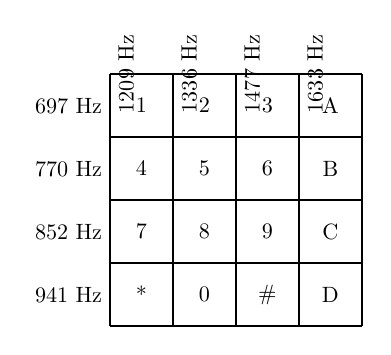
\begin{tikzpicture}[scale=0.8, every node/.style={transform shape}]
                % Grid
                \draw[step=1.0,black,thick] (0,0) grid (4,4);
                % Labels
                \node at (0.5, 3.5) {1}; \node at (1.5, 3.5) {2}; \node at (2.5, 3.5) {3}; \node at (3.5, 3.5) {A};
                \node at (0.5, 2.5) {4}; \node at (1.5, 2.5) {5}; \node at (2.5, 2.5) {6}; \node at (3.5, 2.5) {B};
                \node at (0.5, 1.5) {7}; \node at (1.5, 1.5) {8}; \node at (2.5, 1.5) {9}; \node at (3.5, 1.5) {C};
                \node at (0.5, 0.5) {*}; \node at (1.5, 0.5) {0}; \node at (2.5, 0.5) {\#}; \node at (3.5, 0.5) {D};
                
                % Frequencies
                \node[anchor=east] at (0, 3.5) {697 Hz};
                \node[anchor=east] at (0, 2.5) {770 Hz};
                \node[anchor=east] at (0, 1.5) {852 Hz};
                \node[anchor=east] at (0, 0.5) {941 Hz};
                
                \node[anchor=south, rotate=90] at (0.5, 4) {1209 Hz};
                \node[anchor=south, rotate=90] at (1.5, 4) {1336 Hz};
                \node[anchor=south, rotate=90] at (2.5, 4) {1477 Hz};
                \node[anchor=south, rotate=90] at (3.5, 4) {1633 Hz};
            \end{tikzpicture}
        \end{column}
    \end{columns}
\end{frame}

\begin{frame}{Tone Synthesis \& Export}
    \textbf{Step 1: Signal Generation} \\
    A DTMF signal $x[n]$ is simply the superposition of two sinusoids:
    \[
    x[n] = \sin\left(2\pi f_{\text{low}} \frac{n}{f_s}\right) + \sin\left(2\pi f_{\text{high}} \frac{n}{f_s}\right)
    \]
    where $f_s$ is the sampling rate (typically 8000 Hz).
    
    \vspace{0.5cm}
    \textbf{Step 2: Sequence Assembly}
    \begin{itemize}
        \item To transmit a phone number (e.g., "512"), individual tones are generated and concatenated.
        \item Silent gap buffers (zeros) are inserted between tones to allow the receiver to segment discrete digits.
    \end{itemize}
\end{frame}

\begin{frame}{Signal Segmentation}
    \textbf{Goal:} Isolate active tone regions from continuous recordings (which may contain silence or room noise).
    
    \vspace{0.5cm}
    \textbf{Algorithm:}
    \begin{enumerate}
        \item \textbf{Framing:} Divide the full audio array into 10 ms chunks.
        \item \textbf{RMS Energy:} Calculate the Root Mean Square (RMS) energy for each chunk.
        \item \textbf{Thresholding:} Set a threshold $T = 0.05 \times \max(\text{RMS})$ to separate active tones from the noise floor.
        \item \textbf{Merging:} Track consecutive loud chunks as a single contiguous region $\rightarrow [start, end]$.
    \end{enumerate}
    \vspace{0.3cm}
    \textit{Note: False positives picked up by the low threshold are discarded later by strict spectral validation.}
\end{frame}

\begin{frame}{The Goertzel Algorithm}
    \textbf{Why not FFT?} Computing an entire FFT is wasteful if we only care about 8 specific frequencies.
    
    \vspace{0.5cm}
    \textbf{The Math:}
    The Goertzel algorithm computes a single-bin DFT via a 2nd-order IIR filter. For a target frequency $f_k$:
    \[
    \omega_k = 2\pi \frac{f_k}{f_s} \quad \Rightarrow \quad \text{Coeff} = 2\cos(\omega_k)
    \]
    \textbf{Recurrence Relation:}
    \[
    s[n] = x[n] + \text{Coeff} \cdot s[n-1] - s[n-2]
    \]
    \textbf{Power Output:}
    \[
    |X[k]|^2 = s[N-1]^2 + s[N-2]^2 - \text{Coeff} \cdot s[N-1] \cdot s[N-2]
    \]
    The target frequencies map to conjugate pole pairs $e^{\pm j\omega_k}$ on the unit circle.
\end{frame}

\begin{frame}{Custom Fast Fourier Transform (FFT)}
    \textbf{Implementation:} Radix-2 Cooley-Tukey Algorithm in pure Python.
    
    \vspace{0.5cm}
    \begin{itemize}
        \item \textbf{Zero-Padding:} Input is padded to the next power of 2.
        \item \textbf{Bit Reversal:} Input array indices are sorted in bit-reversed order.
        \item \textbf{Butterfly Operations:} Computed iteratively across $\log_2(N)$ stages.
        \item \textbf{Twiddle Factors:} $W_N^k = e^{-j\frac{2\pi}{N}k}$ applied at each level.
    \end{itemize}
    \vspace{0.5cm}
    While computationally $O(N \log N)$ like standard implementations, running it in pure Python over long live audio buffers poses a performance challenge (solved by isolating analysis to bounded trailing windows).
\end{frame}

\begin{frame}{Enhanced FFT Decoding}
    Raw rectangular-window FFT peak-picking is prone to spectral leakage and bin resolution issues. Dialysis uses an enhanced FFT path:
    
    \vspace{0.5cm}
    \begin{enumerate}
        \item \textbf{Hann Windowing:} Multiplies the tone region by a Hann window to kill spectral leakage.
        \item \textbf{Zero-Padding (2x):} Artificially increases frequency domain bin resolution.
        \item \textbf{Parabolic Peak Interpolation:} Finds the true sub-bin peak by fitting a parabola to the highest magnitude bin and its two neighbors.
        \item \textbf{Tolerance Check:} Snaps the estimated peak to the nearest nominal DTMF frequency (must be within $\pm 2.5\%$).
    \end{enumerate}
\end{frame}

\begin{frame}{Live Decoding Engine (DtmfTracker)}
    Static file thresholds fail on live microphones due to dynamic room noise. We use a \textbf{Temporal State Machine}.
    
    \vspace{0.3cm}
    \begin{itemize}
        \item \textbf{Frame Geometry:} Audio is analyzed in 20 ms frames with a 5 ms hop size.
        \item \textbf{Adaptive Noise Floor:} Min-with-leak tracker. Drops instantly, rises max 10 dB/s.
        \item \textbf{Vectorized Goertzel:} Computes 8 bin powers per frame via a single matrix multiplication.
        \item \textbf{Latch \& Release:} 
        \begin{itemize}
            \item Latches a digit after 6 consecutive agreeing frames (30 ms).
            \item Releases after 4 consecutive disagreeing frames (20 ms).
        \end{itemize}
    \end{itemize}
\end{frame}

\begin{frame}{ITU-T Q.24 Validation}
    Once a tone is latched, it must pass rigorous telecommunication standards to be accepted as genuine DTMF (rejecting speech, music, and noise).
    
    \vspace{0.5cm}
    \textbf{Validation Checks:}
    \begin{enumerate}
        \item \textbf{Dial Tone:} The 350+440 Hz PSTN dial tone pair must not dominate.
        \item \textbf{Twist (Amplitude Ratio):} 
        \begin{itemize}
            \item Forward Twist: Row tone max 15 dB louder than column tone.
            \item Reverse Twist: Column tone max 12 dB louder than row tone.
        \end{itemize}
        \item \textbf{Frequency Offset:} The identified frequency must be the local maximum among $\pm 2.5\%$ neighborhood probes.
        \item \textbf{Harmonic Drop:} The $2^{nd}$ harmonic of either tone must be $\ge 6$ dB below its fundamental (rejects human voice).
    \end{enumerate}
\end{frame}

\begin{frame}{Noise \& Aliasing (Phase 10)}
    Dialysis provides active controls to deliberately break the decoders:
    
    \vspace{0.5cm}
    \begin{columns}
        \begin{column}{0.5\textwidth}
            \textbf{Signal-to-Noise Ratio (SNR)}
            \begin{itemize}
                \item Injects Additive White Gaussian Noise (AWGN) to a specific SNR limit.
                \item Demonstrates decoder resilience (the adaptive gate survives down to $\sim 0$ dB SNR).
            \end{itemize}
        \end{column}
        \begin{column}{0.5\textwidth}
            \textbf{Nyquist-Shannon Aliasing}
            \begin{itemize}
                \item Resampling the signal below $f_s = 3267$ Hz (where $f_{Nyquist} = 1633.5$ Hz) introduces destructive frequency folding.
                \item High-frequency column tones alias into the lower spectrum, permanently destroying the DTMF signature.
            \end{itemize}
        \end{column}
    \end{columns}
\end{frame}

\begin{frame}{Conclusion}
    \begin{center}
        \Large \textbf{Dialysis successfully bridges textbook DSP concepts with robust real-time software engineering.} \\
        \vspace{1cm}
        Thank You!
    \end{center}
\end{frame}

\end{document}
